\documentclass{article}
\usepackage[utf8]{inputenc}
\usepackage{graphicx}
\usepackage{amsmath}
\usepackage{stmaryrd}   % llbracket, rrbracket
\usepackage{siunitx}	% SI units
\usepackage{geometry}
\usepackage{charter}	% betterfont

\geometry{top=1.5cm,bottom=1.5cm, left=2cm, right=2cm}

\begin{document}

\appendix
\section{Linear constraints to model RNA Structure in a linear integer program}
The constraints have been rewritten by us, but are inspired by works like IPknot, Biokop, and RNA-MoIP.

\paragraph{Extended notations} ~ Here we repeat the definition of the variables that we already used in the article, and we use a few more, that also are defined:\\
Let $n$ be the number of nucleotides in the query RNA sequence $s$.\\
Let $M$ be the set of modules that could be inserted in $s$.\\
Let $x$ be a module of $M$, $\|x\|$ be the number of distinct components of $x$, and $p(x)$ the associated score of insertion given by JAR3D or BayesPairing for that motif inserted at a particular position.\\
Let $P_{x,i}$ be the position in $s$ where we can insert the $i$th component of module $x$.\\
As the same module model can be inserted several times in $s$, several different $x$ modules in $M$ may refer to the same theoretical module, but inserted at different positions.\\
Let $k_{x,i}$ be the size in nucleotides of that $i$th component of $x$.\\
Let $y^u_v$ be the \textbf{decision boolean variable} indicating that $s[u]$ and $s[v]$ form a canonical base pairing. According to the standard loop model, we always have $v > u + 3$.\\
Let $C^x_i$ be the \textbf{decision boolean variable} indicating that we do insert the $i$th component of module $x$ at position $P_{x,i}$.


Note that a base pair $y^u_v$ is possible if and only if $v>u+3$, and that we do not need to use two variables $y^u_v$ and $y_{vu}$ for the same pair. 
Then, we have $\sum_{i=4}^n (n-i)$ decision variables ($\approx \frac{1}{2}n^2$ decision variables) of the form $y^u_v$.
Regarding the $C^x_i$, if we have an average insertion of $\nu$ motives by RNA sequence, the motives having in average $\mu$ components, components that can be inserted in average at $\pi$ different positions in $s$,
then we need to add, in average, $\nu \times \mu \times \pi$ decision variables $C^x_i$.

Then, we expect having around $\frac{1}{2}n^2+\nu \mu \pi$ decision variables.

%%%%%%%%%%%%%%%%%%%%%%%%%%%%%%
\paragraph{Constraint to ensure there only is 0 or 1 canonical pairing by nucleotide} ~ 
\begin{equation} \label{constraint:1}
	\sum_{v<u} y^v_u + \sum_{v>u} y^u_v \leq 1 \qquad\qquad \forall u \in \llbracket 1,n \rrbracket
\end{equation}

%%%%%%%%%%%%%%%%%%%%%%%%%%%%%%
\paragraph{Constraints to forbid lonely base pairs} ~
% \begin{equation} \label{constraint:2}
% 	\sum_{v=u}^n y^{u-1}_v - \sum_{v=u+1}^n y^u_v + \sum_{v=u+2}^n y^{u+1}_v \geq 0 \qquad \qquad \forall u \in \llbracket 1,n\rrbracket
% \end{equation}
% \begin{equation} \label{constraint:3}
% 	\sum_{u=1}^{v-2} y^u_{v-1} - \sum_{u=1}^{v-1} y^u_v + \sum_{u=1}^{v} y^u_{v+1} \geq 0 \qquad \qquad \forall v \in \llbracket 1,n\rrbracket
% \end{equation}
% These conditions ensure that if a base pair exists with $s[i]$, 
% one of the adjacent bases is paired too. 
% Equation \ref{constraint:2} is useful if $s[u]$ is paired with $s[v>u]$ (a nucleotide later in the sequence), 
% and equation \ref{constraint:3} if $s[v]$ is paired with $s[u<v]$ (a nucleotide earlier in the sequence).
\begin{equation} \label{constraint:2}
	y^{u-1}_{v+1} - y^u_v + y^{u+1}_{v-1} \geq 0 \qquad \qquad \forall (u,v) \in \{ (u,v) \in \llbracket 1,n\rrbracket^2 \; | \; u + 3 <v \}
\end{equation}
A basepair should be accompanied by one of its neighbours, forming a stable structure stabilized by stacking energies. In theory, this might add up to \( \frac{1}{2}n^2\) constraints, but in practice, this number is very reasonable as
the only decision variables kept are those with probability above a $\theta$ threshold. 
Then, this condition sets to zero "lonely decision variables" who have no neighbour basepair variable allowed.


%%%%%%%%%%%%%%%%%%%%%%%%%%%%%%
\paragraph{Constraint to forbid pairings inside a module component} ~ 
\begin{equation} \label{constraint:4}
	(k_{x,i}-2) \; C^x_i + \sum_{u=P_{x,i}+1}^{P_{x,i}+k_{x,i}-2}\left[ \sum_{v>u} y^u_v + \sum_{v<u} y^v_u \right] \leq (k_{x,i} - 2)
	\qquad \qquad \forall x \in M, i \in \llbracket 1,\|x\| \rrbracket
\end{equation}
If $C^x_i$ is set to 1, then the sum has to be zero. Obviously, this constraint prevents the program to correctly detect pseudoknots of HHH (kissing hairpins) and LL types (kissing higher-order loops), which is a limit of the approach.

%%%%%%%%%%%%%%%%%%%%%%%%%%%%%%
\paragraph{Constraint to forbid component to overlap} ~
\begin{equation} \label{constraint:5}
	\sum_{x \in M} \sum_{i=1}^{\|x\|} C^x_i \times I(P_{x,i}<u<P_{x,i}+k_{x,i}-1) \leq 1 \qquad \qquad \forall u \in \llbracket 1,n \rrbracket
\end{equation}
$I(P_{x,i}<u<P_{x,i}+k_{x,i}-1)$ is a boolean value depending on the condition's truth. Then, whatever the nucleotide $u$, it can be part of a module component only once.

%%%%%%%%%%%%%%%%%%%%%%%%%%%%%%
\paragraph{Constraints to respect the structure of large motives ($\{ x\in M \; | \; \|x\| \geq 2\}$)} ~ 

This constraint ensures that none or all the components of a motif are inserted.
\begin{equation}\label{constraint:6}
	\sum_{i=2}^{\|x\|} C^x_i = (\|x\| - 1) \times C^{x}_{1}	 \qquad \qquad \forall x \in \{ x\in M \; | \; \|x\| \geq 2\}
\end{equation}

And then, we force base pairs between the end of a component and the beginning of the next one:
\begin{equation}\label{constraint:7}
	C^x_1 \leq y^{P_{x,1}}_{P_{x,\|x\|}+k_{x,\|x\|}-1} \qquad \qquad \forall x \in \{ x\in M \; | \; \|x\| \geq 2\}
\end{equation}
\begin{equation}\label{constraint:8}
	C^x_j \leq y^{P_{x,j}+k_{x,j}-1}_{P_{x,j+1}} \qquad \qquad \forall x \in \{ x\in M \; | \; \|x\| \geq 2\}, \forall j \in \llbracket 1,\|x\| \llbracket
\end{equation}

Constraint \ref{constraint:7} binds the first nucleotide of first component to the last one of the last component. 
Constraint \ref{constraint:8} binds the last nucleotide of component $j$ to the first of component $j+1$.

%%%%%%%%%%%%%%%%%%%%%%%%%%%%%%
\paragraph{Facultative constraint to forbid pseudoknots} ~
\begin{equation}\label{constraint:9}
	y^u_v + y^k_l \leq 1 \qquad \qquad \forall u,v,k,l \text{ such as } 1\leq u<k<v<l\leq n
\end{equation}

To limit the number of constraints added, we obviously define the condition for allowed basepairs only ($u + 3 <v$, $k + 3 <l$, $p_{uv} > \theta$, $p_{kl} > \theta$).



%%%%%%%%%%%%%%%%%%%%%%%%%%%%%%
\paragraph{Constraint to forbid a previously found solution} ~ 

As several solutions may result in the same values of the two objectives, we can't forbid the algorithm to search twice the same region of the objective landscape.
We have to explicitly forbid to find again every found solution.\\
We do it by adding iteratively, for every structure $s^*$ found, the following condition :
\begin{equation}\label{constraint:10}
	\sum_{y^u_v \in \{ y^u_v  | y^u_v = 1 \text{ in } s^* \}} (1 - y^u_v) + \sum_{y^u_v \in \{ y^u_v  | y^u_v = 0 \text{ in } s^* \}} y^u_v +
	\sum_{C^x_i \in \{ C^x_i  | C^x_i = 1 \text{ in } s^* \}} (1 - C^x_i) + \sum_{C^x_i \in \{ C^x_i  |C^x_i = 0 \text{ in } s^* \}} C^x_i \geq 1
\end{equation}

It ensures that at least one of the decision variables differs from $s^*$.

%%%%%%%%%%%%%%%%%%%%%%%%%%%%%%%%%%%%%%%%%%%%%%%%%%%%%%%%%%%%%%%%%%%%%%%%%%%%%%%%%%%%%%%%%%%%%%%
%%%%%%%%%%%%%%%%%%%%%%%%%%%%%%%%%%%%%%%%%%%%%%%%%%%%%%%%%%%%%%%%%%%%%%%%%%%%%%%%%%%%%%%%%%%%%%%
\section{Average MCC of the method's variants}
Instead of looking at the best MCC to see if the true structure has been found in the Pareto set, one can look at the average MCC over the Pareto set.

We provide such results to satisfy the reader's curiosity, but this average is hard to interpret. 
The Pareto set is supposed to propose several solutions that could be several meta-stable state, but there is no reason for these states to be close one to another, nor to be close to the "true" structure that has been observed and saved in the database.
A possible interpretation is the average distance of the meta-stable states to the "true" structure, if and only if we assume the predictions are correct.

\hspace{-1cm}
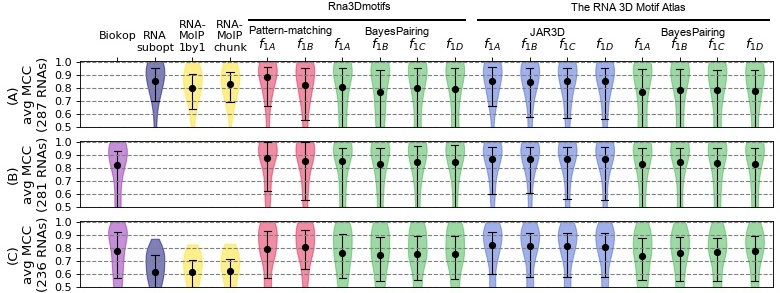
\includegraphics[width=\textwidth]{fig/Benchmark_avg.jpg}

\hspace{-1cm}
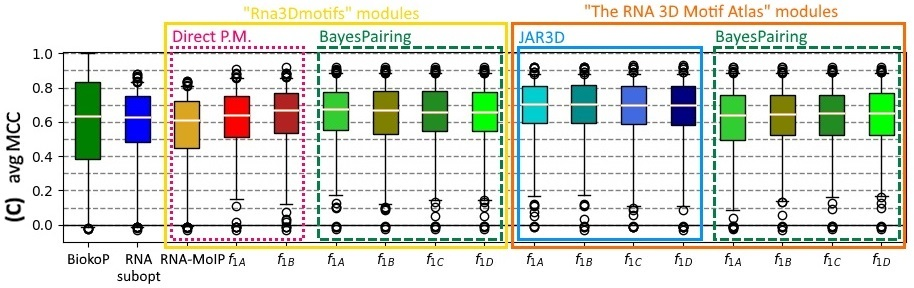
\includegraphics[width=1.05\textwidth]{fig/pseudobase_avg.jpg}

(A) is the RNAstrand dataset for methods which do not support pseudoknots (computations succeeded for all methods for 291 RNAs), (B) is the same dataset but with pseudoknot support (294 RNAs), and (C) is the Pseudobase dataset of 264 RNAs.

%%%%%%%%%%%%%%%%%%%%%%%%%%%%%%%%%%%%%%%%%%%%%%%%%%%%%%%%%%%%%%%%%%%%%%%%%%%%%%%%%%%%%%%%%%%%%%%
%%%%%%%%%%%%%%%%%%%%%%%%%%%%%%%%%%%%%%%%%%%%%%%%%%%%%%%%%%%%%%%%%%%%%%%%%%%%%%%%%%%%%%%%%%%%%%%
\section{Study cases results}
Here we provide the structures and statistics of the 3 well known RNAs that we studied in detail.

\subsection{General statistics}

The first line in Table \ref{Tab:01} gives the results for E.\textit{coli} tRNA Gln  (PDB\_00376), the second line for the glycine riboswitch (PDB\_01023), and the third for the human telomerase's pseudoknot (PDB\_00857). We observe that the best structure is often the same accross the different objective functions $f_{1A}, f_{1B}, f_{1C}, f_{1D}$, but the rest of the set can be different in number of solutions and diversity.

\begin{table*}[h]
\caption{Best MCC results for study cases. Pseudoknots are allowed. \label{Tab:01}}
\vspace{5mm}
\begin{tabular}{@{}r|lll|@{}} & RNAsubopt & RNA-MoIP & BiokoP \\
 & & & \\\hline
PDB\_00376 & 0.68 & 0.68 & 0.67 \\
PDB\_01023 & 0.86 & 0.86 & 0.59 \\
PDB\_00857 & 0.77 & 0.77 & 1.0 \\
\end{tabular}
\vspace{5mm}
\vfill

\begin{tabular}{@{}r|llll|@{}} &  Rna3Dmotifs & Rna3Dmotifs & RNA 3D Motif Atlas & RNA 3D Motif Atlas\\
 & + Direct P.M. & + BayesPairing & + JAR3D & + BayesPairing \\\hline
PDB\_00376 &  0.72 (A,B) & 0.74 (B,C,D), 0.71 (A) & 0.74 (A,C,D), 0.72 (B) & 0.76 (\textit{all})\\
PDB\_01023 &  0.79 (A,B) & 0.29 (\textit{all}) & 0.82 (\textit{all}) & 0.82 (\textit{all})\\
PDB\_00857 &  0.97 (B), 0.77 (A) & 0.97 (\textit{all}) & 0.97 (\textit{all}), & 0.97 (\textit{all})\\
\end{tabular}
\end{table*}

Detailed results are given below for each RNA. The number of solutions and computation times are also reported. Note that these cases are small RNAs, resulting in both small number of solutions and small times. The times are the "Real" time spent, therefore you should use the same 16-thread CPU to reproduce them, because there are several multi-threaded parts in the process. They also are very dependant of the I/O delays. Especially with methods reading modules from disk, you may want to use a very fast storage device (e.g. NVMe SSD NAND storage) to increase the speed.

\newpage
%%%%%%%%%%%%%%%%%%%%%%%%%%%%%%%%%%%%%%%%%%%%%%%%%%%%%%%%%%%%%%%%%%%%%%%%%%%%%%%%%%%%%%%%%%%%%%%
\subsection{E. coli's Gln tRNA}
\paragraph{Sequence (FASTA format)} ~ 

\texttt{>>'CRYSTAL STRUCTURE OF A TIGHT-BINDING GLUTAMINE TRNA BOUND TO GLUTAMINE AMINOACYL TRNA SYNTHETASE ' (PDB 00376)\\
GGGGUAUCGCCAAGCGGUAAGGCACCGGAUUCUGAUUCCGGAGGUCGAGGUUCGAAUCCUCGUACCCCAGCCA}

\paragraph{Referenced "true" structure in RNA-Strand (PDB 00376)} ~ 

\texttt{((((((..(((.........)))((((((((...))))))))...(((((.......))))))))))).....}

\paragraph{Best prediction results} ~ 

{\scriptsize
\begin{tabular}{rlccr}
Method & Best secondary structure & best MCC & N solutions & time (s)\\
\hline
True structure:	& \texttt{((((((..(((.........)))((((((((...))))))))...(((((.......))))))))))).....} & & & \\
RNAsubopt:&	 \texttt{(((((((.(((....)))..(((.(((((.......)))))..)))((((.......))))))))))).....} &0.68 &4 & 0.01\\
Biokop	:&	 \texttt{[[[[[[((((...))))...(((.((((([[[....)))))....(((((...]]].)))))]]]]]].))).}& 0.67 &30& 10.3\\
RNA-MoIP	:&	 \texttt{((((((..((......))...((.(((((.......)))))..))..((.........))..)))))).....}& 0.67 &4& 0.01+5.0\\
Direct P.M.-A	:&	 \texttt{((((((((((...))))....((.(((((.......)))))..))(((((.......))))))))))).....} &0.72 &8& 7.7\\
Direct P.M.-B	:	& \texttt{((((((((((...))))....((.(((((.......)))))..))(((((.......))))))))))).....} &0.72 &11& 7.9\\
BayesPairing-A:&	 \texttt{(((((((((((....)))......(((((.......))))).)).((((.........)))))))))).....} &0.71 &7& 74+9.9\\
BayesPairing-B:&	 \texttt{(((((((((((....)))......(((((.......))))).)).(((((.......))))))))))).....} &0.74 &8& 74+15.5\\
BayesPairing-C:	& \texttt{(((((((((((....)))......(((((.......))))).)).(((((.......))))))))))).....} &0.74 &9& 74+8.6\\
BayesPairing-D:	& \texttt{(((((((((((....)))......(((((.......))))).)).(((((.......))))))))))).....} &0.74 &10& 74+9.2\\
JAR3D-A	:	& \texttt{(((((((((((....)))......(((((.......))))).)).(((((.......))))))))))).....} &0.74 &3& 0.01+1.3+7.9\\
JAR3D-B	:	& \texttt{((((((((((...))))....((.(((((.......)))))..))(((((.......))))))))))).....} &0.72 &3& 0.01+1.3+8.9\\
JAR3D-C	:&	 \texttt{(((((((((((....)))......(((((.......))))).)).(((((.......))))))))))).....} &0.74 &5& 0.01+1.3+7.7\\
JAR3D-D	:&	 \texttt{(((((((((((....)))......(((((.......))))).)).(((((.......))))))))))).....} &0.74 &5& 0.01+1.3+7.9\\
BGSU-BPairing-A:	& \texttt{((((((((.......))....((.(((((.......)))))..))(((((.......))))))))))).....} &0.76 &6& 61+8.7\\
BGSU-BPairing-B:	& \texttt{((((((((.......))....((.(((((.......)))))..))(((((.......))))))))))).....} &0.76 &10& 61+12.1\\
BGSU-BPairing-C:&	 \texttt{((((((((.......))....((.(((((.......)))))..))(((((.......))))))))))).....} &0.76 &4& 61+7.5\\
BGSU-BPairing-D:	& \texttt{((((((((.......))....((.(((((.......)))))..))(((((.......))))))))))).....} &0.76& 4& 61+7.2\\
\end{tabular}}

\paragraph{Notes} ~

Note that BiokoP inserts a false-positive pseudoknot, while the Biorseo variants do not. If we look at our two recommended methods, here is an example of difference in the number of solutions : Biorseo+Rna3Dmotifs+Direct Pattern Matching + function B return 11 solutions, while Biorseo+The RNA 3D Motif Atlas+JAR3D+function B returns only 3, with the same best MCC of 0.72.

%%%%%%%%%%%%%%%%%%%%%%%%%%%%%%%%%%%%%%%%%%%%%%%%%%%%%%%%%%%%%%%%%%%%%%%%%%%%%%%%%%%%%%%%%%%%%%%
\subsection{G Riboswitch}

\paragraph{Sequence (FASTA format)} ~ 

\texttt{>  'GUANINE RIBOSWITCH U22C, A52G MUTANT BOUND TO HYPOXANTHINE ' (PDB 01023)\\
GGACAUACAAUCGCGUGGAUAUGGCACGCAAGUUUCUGCCGGGCACCGUAAAUGUCCGACUAUGUCCa}

\paragraph{Referenced "true" structure in RNA-Strand (PDB 01023)} ~ 

\texttt{(((((((...(((((((.[[..[[)))))))........((((((]]...]]))))))..))))))).}

\paragraph{Best prediction results} ~ 

{\scriptsize
\begin{tabular}{rlccr}
Method & Best secondary structure & best MCC & N solutions & time (s)\\
\hline
True structure:	 & \texttt{(((((((...(((((((.[[..[[)))))))........((((((]]...]]))))))..))))))).} & & & \\
RNAsubopt:	 & \texttt{(((((((.....(((((.......)))))..........((((((.......))))))..))))))).} & 0.86 & 3 & 0.01 \\
Biokop	:	 & \texttt{(((((([[[.[[(((((]][[[[[))))).(((...[[[(((]]]]]]]]..]]])))))))))))).} & 0.59 & 4 & 58.2 \\
RNA-MoIP	:	 & \texttt{(((((((.....(((((.......)))))..........(((((.........)))))..))))))).} & 0.84 & 3 & 0.01+4.1\\
Direct P.M.-A	:	 & \texttt{(((((((.....(((((.......)))))..((....))(((((.........)))))..))))))).} & 0.79 & 15 & 4.3 \\
Direct P.M.-B	:	 & \texttt{((((.((.....(((((.......))))).((...))..((((((.......))))))..)).)))).} & 0.79 & 18 & 9.0 \\
BayesPairing-A:	 & \texttt{...............(((((((((.((....))......((((((.......)))))).)))))))))} & 0.29 & 4 & 53+8.3\\
BayesPairing-B:	 & \texttt{...............(((((((((.((....))......((((((.......)))))).)))))))))} & 0.29 & 4 & 53+8.4\\
BayesPairing-C:	 & \texttt{...............(((((((((.((....))......((((((.......)))))).)))))))))} & 0.29 & 3 & 53+5.8\\
BayesPairing-D:	 & \texttt{...............(((((((((.((....))......((((((.......)))))).)))))))))} & 0.29 & 3 & 53+5.6\\
JAR3D-A	:	 & \texttt{(((((((.....(((((.......)))))..((....))((((((.......))))))..))))))).} & 0.82 & 4 & 0.01+1.2+30.3\\
JAR3D-B	:	 & \texttt{(((((((.....(((((.......)))))..((....))((((((.......))))))..))))))).} & 0.82 & 5 & 0.01+1.2+23.8\\
JAR3D-C	:	 & \texttt{(((((((.....(((((.......)))))..((....))((((((.......))))))..))))))).} & 0.82 & 2 & 0.01+1.2+4.7\\
JAR3D-D	:	 & \texttt{(((((((.....(((((.......)))))..((....))((((((.......))))))..))))))).} & 0.82 & 2 & 0.01+1.2+4.6\\
BGSU-BPairing-A:	 & \texttt{(((((((.....(((((.......)))))..((....))((((((.......))))))..))))))).} & 0.82 & 9 & 58+6.2\\
BGSU-BPairing-B:	 & \texttt{(((((((.....(((((.......)))))..((....))((((((.......))))))..))))))).} & 0.82 & 9 & 58+8.4\\
BGSU-BPairing-C:	 & \texttt{(((((((.....(((((.......)))))..((....))((((((.......))))))..))))))).} & 0.82 & 9 & 58+6.7\\
BGSU-BPairing-D:	 & \texttt{(((((((.....(((((.......)))))..((....))((((((.......))))))..))))))).} & 0.82 & 9 & 58+8.1\\
\end{tabular}}

\paragraph{Notes} ~

On one side, here again, BiokoP predicts too many knots. The RNA only contains one kissing-hairpin HHH pseudoknot. On the other side, as expected, this HHH knot is not detected by Biorseo.

%%%%%%%%%%%%%%%%%%%%%%%%%%%%%%%%%%%%%%%%%%%%%%%%%%%%%%%%%%%%%%%%%%%%%%%%%%%%%%%%%%%%%%%%%%%%%%%
\subsection{Human telomerase's RNA pseudoknot}

\paragraph{Sequence (FASTA format)} ~ 

\texttt{>  'SOLUTION STRUCTURE OF THE P2B-P3 PSEUDOKNOT FROM HUMAN TELOMERASE RNA ' (PDB 00857)\\
GGGCUGUUUUUCUCGCUGACUUUCAGCCCCAAACAAAAAAGUCAGCA}

\paragraph{Referenced "true" structure in RNA-Strand (PDB 00857)} ~ 

\texttt{[[[[[[........(((((((((]]]]]]........))))))))).}

\paragraph{Best prediction results} ~ 

{\scriptsize
\begin{tabular}{rlccr}
Method & Best secondary structure & best MCC & N solutions & time (s)\\
\hline
True structure:	 & \texttt{[[[[[[........(((((((((]]]]]]........)))))))))} & & & \\
RNAsubopt:	 & \texttt{..............(((((((((..............))))))))).} &  0.77 & 3 & 0.06\\
Biokop	:	 & \texttt{[[[[[[........(((((((((]]]]]]........))))))))).} &  1.00 & 1 & 4.7\\
RNA-MoIP	:	 & \texttt{..............(((((((((..............))))))))).} &  0.77 & 3 & 0.06+3.3\\
Direct P.M.-A	:	 & \texttt{..............(((((((((..............))))))))).} &  0.77 & 3 & 0.8\\
Direct P.M.-B	:	 & \texttt{[[[[[[........((((((((.]]]]]].........)))))))).} &  0.97 & 7 & 0.7\\
BayesPairing-A:	 & \texttt{[[[[[[........((((((((.]]]]]].........)))))))).} &  0.97 & 2 & 71+1.0\\
BayesPairing-B:	 & \texttt{[[[[[[........((((((((.]]]]]].........)))))))).} &  0.97 & 2 & 71+0.6\\
BayesPairing-C:	 & \texttt{[[[[[[........((((((((.]]]]]].........)))))))).} &  0.97 & 2 & 71+0.6\\
BayesPairing-D:	 & \texttt{[[[[[[........((((((((.]]]]]].........)))))))).} &  0.97 & 2 & 71+0.6\\
JAR3D-A	:	 & \texttt{[[[[[[........((((((((.]]]]]].........)))))))).} &  0.97 & 2 & 0.06+1.3+0.8\\
JAR3D-B	:	 & \texttt{[[[[[[........((((((((.]]]]]].........)))))))).} &  0.97 & 2 & 0.06+1.3+0.6\\
JAR3D-C	:	 & \texttt{[[[[[[........((((((((.]]]]]].........)))))))).} &  0.97 & 2 & 0.06+1.3+0.6\\
JAR3D-D	:	 & \texttt{[[[[[[........((((((((.]]]]]].........)))))))).} &  0.97 & 2 & 0.06+1.3+0.6\\
BGSU-BPairing-A:	 & \texttt{[[[[[[........((((((((.]]]]]].........)))))))).} &  0.97 & 2 & 57.7+0.5\\
BGSU-BPairing-B:	 & \texttt{[[[[[[........((((((((.]]]]]].........)))))))).} &  0.97 & 2 &  57.7+0.5\\
BGSU-BPairing-C:	 & \texttt{[[[[[[........((((((((.]]]]]].........)))))))).} &  0.97 & 2 & 57.7+0.5\\
BGSU-BPairing-D:	 & \texttt{[[[[[[........((((((((.]]]]]].........)))))))).} &  0.97 & 2 & 57.7+0.5\\
\end{tabular}}


\paragraph{Notes} ~

The methods which support pseudoknots are able to predict it correctly.
\end{document}